\documentclass{article}
\usepackage{longtable}
\usepackage{makecell}
\usepackage{float}
\usepackage{graphicx}
\usepackage{bm}
\usepackage{amsmath}
\usepackage{placeins}
\usepackage{threeparttable} 
\usepackage{multirow}
\usepackage{aligned-overset}
\usepackage[slantfont,boldfont]{xeCJK}
\usepackage{fontspec}
\counterwithin{figure}{section}
\renewcommand{\arraystretch}{1.5}
\setCJKmainfont{SimSun}
\setmainfont{SimSun}
\setsansfont{SimSun}

\title{薄透镜焦距测量\\及自组显微镜、望远镜实验报告}
\author{2411545 邱凯锐}
\date{2025.3.24}

\begin{document}
\maketitle
\section{实验目的}
\begin{itemize}
    \item 1.掌握透镜焦距的简单测量方法;
    \item 2.掌握显微镜和望远镜的基本结构、工作原理及其调节和使用方法。
\end{itemize}
\section{实验原理}
\subsection{透镜焦距的测量}
1.\textbf{自准直法}\\
\hspace*{2em}自准直是光学实验中经常采用的一种实验技术,自准直技术在平行光管和测量望远镜的调整、测量球面和非球面的面型以及测量透镜或光学系统的焦距等方面有着广泛应用。\\
\hspace*{2em}无限远的物镜透镜成像,像处在透镜的角平面上。自准直法测量透镜焦距就是首先利用待测透镜自身产生一个位于无限远的物,再用待测透镜对它成像,通过测量像与透镜之间的距离来确定透镜的焦距。准直技术在光学实验中通常是指产生平行光束或获得处于无限远的物的方法。\\
\hspace*{2em}自准直法测量透镜焦距的原理如Figure 2.1所示。当物\(y\)位于透镜的焦平面上时,经透镜\(L\)和平面反射镜所组成的光学系统后,当在焦平面上成一与物等大的倒立实像时,物到透镜中心的距离就是透镜的焦距。
\\
2.\textbf{位移法}\\
\hspace*{2em}位移法又称贝塞尔法或二次成象法。测量原理如Figure 2.1所示。首先选定物象间的距离\(A\)。如果,透镜在这个距离间能有两个成像位置,透镜的两个成像位置之间的距离为\(d\)。从Figure 2.1可以看到两次成像的物距和象距与\(A\)、\(d\)有以下关系,
\begin{equation}
    S_1'-S_2'=d, S_1-S_2=d,S_1'-S_1=A,S_2'-S_2=A
\end{equation}
考虑到薄透镜的成象公式:
\begin{equation}
    \frac{1}{S'}-\frac{1}{S}=\frac{1}{f'}
\end{equation}
可以得到,
\begin{equation}
    S_1=-S_2'=-\frac{A-d}{2},S_1'=-S_2=\frac{A+d}{2}
\end{equation}
将式(2)代入式(3)有
\begin{equation}
    \frac{1}{\frac{A-d}{2}}-\frac{1}{\frac{A+d}{2}}=\frac{1}{f'}
\end{equation}
得到:
\begin{equation}
    d=\sqrt{A(A-4f')}
\end{equation}
由此式可知,在固定物象距离\(A\)的情况下,如果透镜有两个成实象的位置,\(A\)必须大于\(4\)倍焦距。\\
\hspace*{2em}通过测量得到\(A\)和\(d\)后,由式(4)可知,透镜的焦距为
\begin{equation}
    f'=\frac{A^2-d^2}{4A}
\end{equation}
\begin{figure}[ht]
    \centering
    \begin{minipage}{0.45\textwidth} % 调整宽度为总宽度的45%
        \centering
        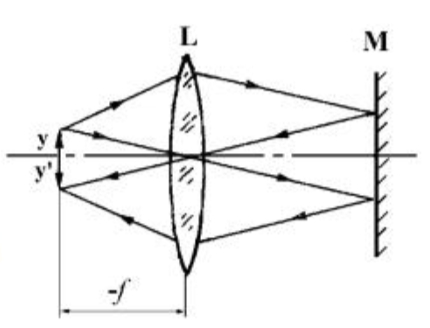
\includegraphics[width=6cm]{2.1.1.png} % 替换为你的图片路径
        \caption{自准直法}
    \end{minipage}\hfill
    \centering
    \begin{minipage}{0.45\textwidth} % 调整宽度为总宽度的45%
        \centering
        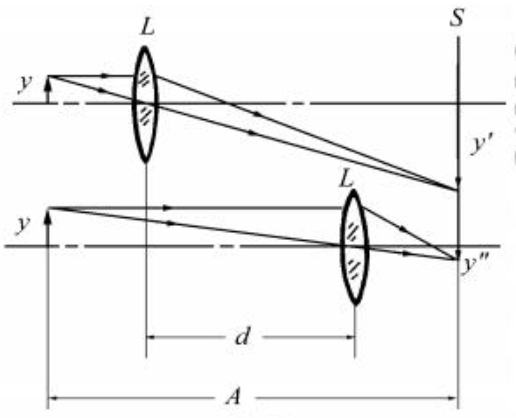
\includegraphics[width=6cm]{2.1.2.png} % 替换为你的图片路径
        \caption{位移法}
    \end{minipage}\hfill
\end{figure}
\subsection{光学显微镜、望远镜}
1.\textbf{显微镜}\\
\hspace*{2em}最基本的显微镜是由目镜和物镜组成:靠近被观察物体的是物镜;靠近眼睛的是目镜。目镜和物镜可以是单透镜,但在多数情况下,为减小各种象差,提高成象质量,物镜和目镜均由透镜组组成。图\ref{fig:3}是显微镜的光路图。被观察的物\(y_1\)处在物镜前面一倍焦距和二倍焦距之间,它经物镜成一放大的倒立实象\(y_2\),位于目镜的焦点内侧或在目镜的焦平面上,通过目镜后成一正立的虚象\(y_3\)于明视距离处(\(D = 250mm\))或无限远处。\\
\hspace*{2em}通常所提到的显微镜和望远镜的放大倍数是指视角放大率。人眼所能分辨的物体细节,取决于它在视网膜上象的大小,而此象的大小又是由物体对人眼的张角,即视角\(\omega\)决定。
\begin{equation}
    \tan \omega =\frac{y}{l}
\end{equation}
\begin{figure}[h]
    \centering
    \begin{minipage}{0.45\textwidth} % 调整宽度为总宽度的45%
        \centering
        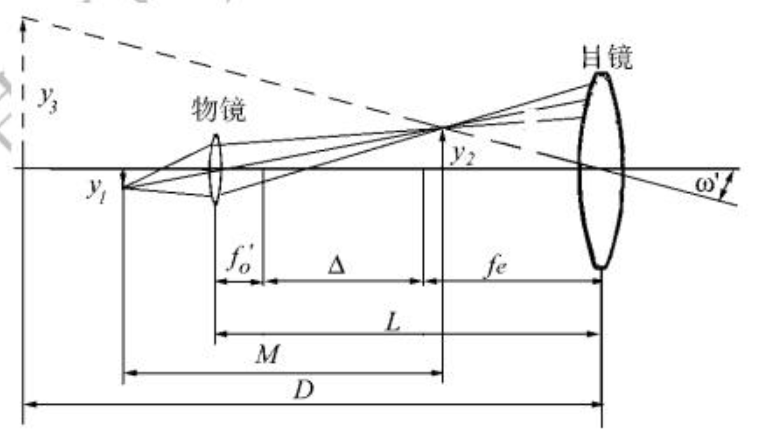
\includegraphics[width=6cm]{2.2.1.png} % 替换为你的图片路径
        \caption{显微镜的工作原理}
    \end{minipage}\hfill
    \centering
    \begin{minipage}{0.45\textwidth} % 调整宽度为总宽度的45%
        \centering
        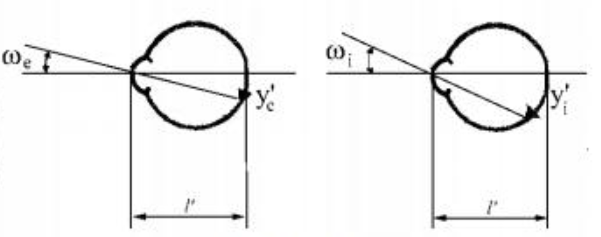
\includegraphics[width=6cm]{2.2.2.png} % 替换为你的图片路径
        \caption{视角放大率}
    \end{minipage}\hfill
\end{figure}
\hspace*{2em}式中,\(y\)为物体的大小;\(l\)为物体到人眼的距离。人眼的分辨率极限为\(1'\)左右。所以人眼能分辨物体细节的条件为
\begin{equation}
    \tan \omega =\frac{y}{l} \geq 0.0003
\end{equation}
\hspace*{2em}当物体对人眼视角小于 \(1'\)时,若要看清它,简单的方法就需要借助于光学仪器。通过光学仪器后在视网膜上成的象大于用眼睛直接看该物时所成的象,固(此处应为“故”)产生了放大的感觉。视角放大率的定义为\\
\begin{equation}
    \Gamma=\frac{y_i'}{y_e'}=\frac{l'\tan\omega_i}{l'\tan\omega_e}=\frac{\tan\omega_i}{\tan\omega_e}
\end{equation}
眼睛看到物体时,物体位于眼前明视距离处,所以:
\begin{equation}
    \tan \omega_e=\frac{y_i}{250}
\end{equation}
由Figure 2.3,可知显微镜观看的视场角$\omega_i$等于显微镜的象方视角$\omega'$,并且有:
\begin{equation}
    \tan\omega_i=\tan\omega'=\frac{y_2}{f_e}
\end{equation}
所以由式(9)可知,显微镜的视角放大率为
\begin{equation}
    \Gamma=\frac{\tan\omega_i}{\tan\omega_e}=\frac{y_2/f_e'}{y_1/250}=\beta_o\cdot\Gamma_e
\end{equation}
又
\begin{equation*}
    \beta_o=-\frac{\Delta}{f_o'}
\end{equation*}
所以
\begin{equation}
    \Gamma=-\frac{\Delta}{f_o'}\frac{250}{f_e'}
\end{equation}
\hspace*{2em}由式\((12)\)可以看到,显微镜的视角放大率等于它的物镜的垂轴放大率和目镜的视角放大率的积。所以将不同倍率的目镜和物镜组合可以很方便地得到显微镜的多种放大倍率。多数显微镜都配有三组不同倍率的目镜和三组不同倍率的物镜。

为保证在更换目镜和物镜时不需要重新调焦就能看到清楚的象(最多辅以微动调焦),显微镜对其光学机械尺寸有如下要求:

机械筒长:  取下物镜和目镜,剩下的镜筒上下端面间的长度为显微镜的机械筒长。

光学筒长:  光学筒长为显微镜的光学间隔\(\Delta\),它随物镜的焦距 \(f_{o}\) 的不同而不同,但在显微镜中要求由物面到物镜的象面的共轭距离 \(M\) 保持不变。即显微镜要满足齐焦条件。\\
2.\textbf{望远镜}\\
\hspace*{2em}当位于远处物体的细节对眼睛的视角小于人眼的分辨极限时,人们必须借助光学仪器才能分辨它。这类光学仪器就是望远镜。\\
\hspace*{2em}简单的望远镜是由两个透镜组成一个光学间隔为零的光学系统。它同显微镜一样,两个透镜分别作为目镜和物镜。望远镜有两种基本类型:开普勒望远镜和伽利略望远镜。开普勒望远镜的目镜和物镜均为正透镜。伽利略望远镜目镜是负透镜(凹透镜),而物镜是正透镜。\\
\hspace*{2em}Figure 2.5是开普勒望远镜调焦于无限远时的光路图。物镜将无限远处的物体在其焦平面上成一倒立实象,然后由目镜将此实象放大,使之在无限远处,供人眼观察。由Figure 2.5可知,望远镜的视角放大率为
\begin{equation}
    \Gamma=\frac{\tan \omega_i}{\tan \omega_e}=-\frac{f_e'}{f_o'}
\end{equation}
\begin{figure}[h]
    \centering
    \begin{minipage}{0.45\textwidth} % 调整宽度为总宽度的45%
        \centering
        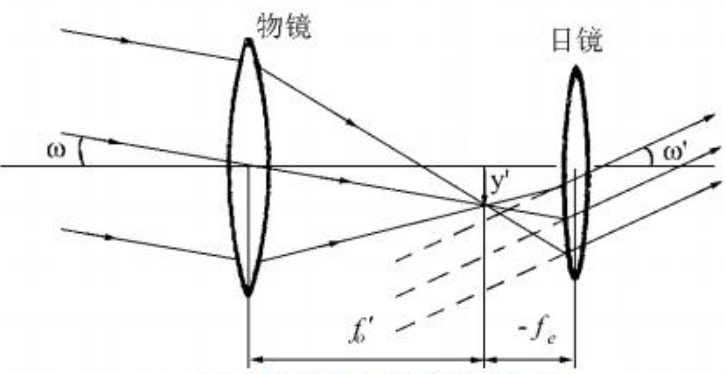
\includegraphics[width=6cm]{2.2.3.png} % 替换为你的图片路径
        \caption{开普勒望远镜}
    \end{minipage}\hfill
    \centering
    \begin{minipage}{0.45\textwidth} % 调整宽度为总宽度的45%
        \centering
        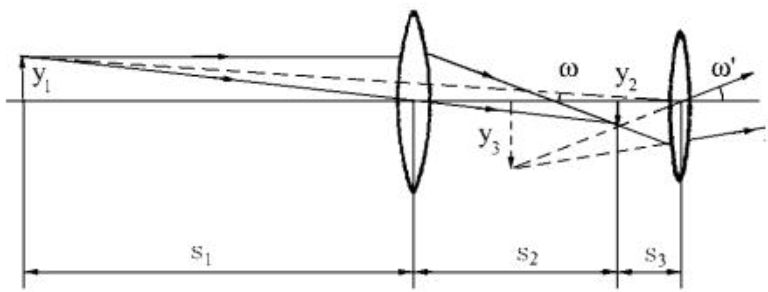
\includegraphics[width=6cm]{2.2.4.png} % 替换为你的图片路径
        \caption{望远镜光路}
    \end{minipage}\hfill
\end{figure}
\\
\hspace*{2em}由此式可见,要使\(\Gamma > 1\),则物镜的焦距要大于目镜的焦距。视角放大率为负说明用开普勒望远镜观察物体时,人眼所看到的是倒象,在使用中很不方便。为此,实用开普勒望远镜必须在物镜和目镜间加入转象系统,使人眼观察到的为正象。对于伽利略望远镜,由于目镜使用了负透镜,它视角放大率是正的,即伽利略望远镜在不用转象系统的情况下,直接观察的就是正象。伽利略望远镜与开普勒望远镜相比,在相同的视角放大率时,不但体积小而且重量轻。但它也有一致命的缺点,由于目镜到物镜的距离小于物镜的焦距,所以在物镜与目镜的共焦面上的象为虚象,故伽利略望远镜中不能安置用于测量的分划板,使它的用途受到了极大的限制。目前伽利略望远镜主要用于民用和激光扩束。而开普勒望远镜可以安置分划板,它目前在计量仪器和军用光学仪器中得到广泛应用。\\
\hspace*{2em}望远镜的视场角为 \(2\omega\),由式\((14)\)可知,望远镜的视角放大率越大其视场角越小。使用高倍数望远镜带来的问题是对准比较困难。\\
\hspace*{2em}在许多情况下,用望远镜所观察的物体并非处于无限远,这时通过改变物镜和目镜之间距离进行调焦,使物体通过物镜所成的实象位于目镜的物方焦平面以里,再经目镜在明视距离外成一虚象。其光路如Figure 2.6所示。这时被观察物体对眼睛的视角为
\begin{equation}
    \tan \omega_e=\tan \omega=\frac{y_i}{S_1+S_2+S_3}
\end{equation}
通过望远镜后视角为
\begin{equation}
    \tan \omega_i=\tan \omega'=\frac{y_2}{S_3}
\end{equation}
又$y_2/y_2=S_2/S_1$,所以望远镜在观察有限远物体时视角放大率为
\begin{equation}
    \Gamma=\frac{\tan \omega_i}{\tan \omega_e}=\frac{S_2(S_1+S_2+S_3)}{S_1S_3}
\end{equation}
\section{实验设备}
\begin{itemize}
    \item 1.5m光具座
    \item 可调节光源$\times 2$
    \item 平面镜
    \item 分化板
    \item 半透半反镜
    \item 薄透镜(大中小三种规格),,透镜架
\end{itemize}
\section{实验内容}
\hspace*{2em}实验前先调节各器件高度,使得光学系统共轴。
\subsection{测量透镜焦距}
\hspace*{2em}测量大、中透镜的焦距,小透镜焦距太小,暂且不测量,其焦距为20.0mm。\\
\hspace*{1em}1.\textbf{自准直法}\\
\hspace*{2em}按照原理图摆放各元件,调节透镜与光源之间的距离,使得板上呈现等大倒立的实象,此时透镜与光源之间的距离即为透镜焦距。\\
\hspace*{1em}2.\textbf{位移法}\\
\hspace*{2em}按照原理图摆放各元件,先确定物象距离$A$(注意满足$A\geq 4f'$),调节透镜位置,记录两次成象的位置$d_1$、$d_2$,并计算两次成象位置的距离$d$以及焦距$f'$。重复实验三次,计算平均值$\overline{f'}$\\
\subsection{自组显微镜并测量其视角放大率}
\hspace*{2em}选择合适的透镜作显微镜的物镜和目镜。固定两透镜间距离为\(180mm\),观察作为物的分划板。\\
\hspace*{2em}为估测显微镜的放大率,在目镜\(L_{e}\)后面放置一个与光轴成\(45^{\circ}\)的半透半反镜,并在与光轴垂直方向上相距\(25cm\)处放置分划板\(S_{2}\),分划板\(S_{1}\)、\(S_{2}\)是完全相同的。此时,眼睛可以同时看到\(S_{1}\)经过显微镜放大的象和\(S_{2}\)未放大的象。稍许调节\(S_{1}\)的位置,使两个象之间无视差时,从对应刻线距离测定显微镜的视角放大率。
\begin{figure}[h]
    \centering
    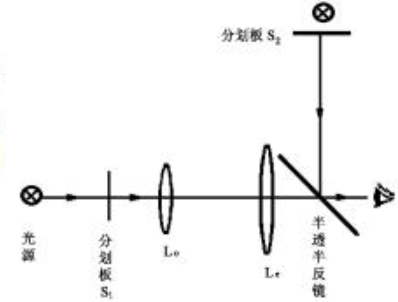
\includegraphics[width=7cm]{2.4.1.png} % 替换为你的图片路径
    \caption{估测显微镜方法倍数}
\end{figure}
\subsection{自组望远镜并计算其视角放大率}
\hspace*{2em}选择焦距合适的两块透镜做望远镜的物镜和目镜。使作为物的分划板和望远镜目镜之间距离在导轨上达到最大,通过移动目镜使望远镜对分划板能成清楚的象。测量\(S_{1}\)、\(S_{2}\)、\(S_{3}\),并计算视角放大率。
\section{实验数据}
\subsection{测量透镜焦距——位移法}
\begin{longtable}{cccccc}
    %\centering
    \caption{大透镜实验数据}
    \label{table:longtable_example} \\
    % 下面是表头
    \hline  组别 & $A$/mm & $d_1$/mm & $d_2$/mm & $d$/mm & $f'$/mm\\ \hline 
    \endfirsthead
    % 下面数字3的意思是表格的列数
    \multicolumn{6}{c}%
    {{continued from previous page}} \\
    \hline  组别 & $A$/mm & $d_1$/mm & $d_2$/mm & $d$/mm & $f'$/mm\\ \hline 
    % 注意这里把表头复制了一遍,因为在新的页面也会展示一下表头,不然表格不方便阅读
    \endhead
    \hline \multicolumn{6}{r}{{Continued on next page}} \\ \hline
    \endfoot
    \hline \hline
    \endlastfoot
    1 & 900  & 395.0 & 771.0 & 376   & 185.7 \\
    2 & 950  & 381.0 & 823.5 & 442.5 & 186.0 \\
    3 & 1000 & 375.0 & 884.0 & 509   & 185.2  \\ \hline
\end{longtable}
计算得$\overline{f_{大}'}=185.6 mm$

\begin{longtable}{cccccc}
    %\centering
    \caption{中透镜实验数据}
    \label{table:longtable_example} \\
    % 下面是表头
    \hline  组别 & $A$/mm & $d_1$/mm & $d_2$/mm & $d$/mm & $f'$/mm\\ \hline 
    \endfirsthead
    % 下面数字3的意思是表格的列数
    \multicolumn{6}{c}%
    {{continued from previous page}} \\
    \hline  组别 & $A$/mm & $d_1$/mm & $d_2$/mm & $d$/mm & $f'$/mm\\ \hline 
    % 注意这里把表头复制了一遍,因为在新的页面也会展示一下表头,不然表格不方便阅读
    \endhead
    \hline \multicolumn{6}{r}{{Continued on next page}} \\ \hline
    \endfoot
    \hline \hline
    \endlastfoot
    1 & 250 & 263.0 & 380.0 & 117 & 48.8 \\
    2 & 300 & 260.0 & 435.0 & 175 & 49.5 \\
    3 & 350 & 258.0 & 492.0 & 234 & 48.4  \\ \hline
\end{longtable}
计算得$\overline{f_{中}'}=48.9 mm$
\subsection{自组显微镜}
\begin{longtable}{cccccc}
    %\centering
    \caption{自组显微镜实验数据}
    \label{table:longtable_example} \\
    % 下面是表头
    \hline  $f_o'$ & $f_e'$/mm & $L$/mm & $\Delta$/mm & $\Gamma_{估测}$ & $\Gamma_{计算}$\\ \hline 
    \endfirsthead
    % 下面数字3的意思是表格的列数
    \multicolumn{6}{c}%
    {{continued from previous page}} \\
    \hline  $f_o'$ & $f_e'$/mm & $L$/mm & $\Delta$/mm & $\Gamma_{估测}$ & $\Gamma_{计算}$\\ \hline 
    % 注意这里把表头复制了一遍,因为在新的页面也会展示一下表头,不然表格不方便阅读
    \endhead
    \hline \multicolumn{6}{r}{{Continued on next page}} \\ \hline
    \endfoot
    \hline \hline
    \endlastfoot
    20.0 & 48.9 & 180.0 & 111.1 & 28 & 28.4 \\\hline
\end{longtable}

\subsection{自组望远镜}
\begin{longtable}{cccccc}
    %\centering
    \caption{自组望远镜实验数据}
    \label{table:longtable_example} \\
    % 下面是表头
    \hline  $f_o'$ & $f_e'$/mm & $S_1$/mm & $S_2$/mm & $S_3$ & $\Gamma_{计算}$\\ \hline 
    \endfirsthead
    % 下面数字3的意思是表格的列数
    \multicolumn{6}{c}%
    {{continued from previous page}} \\
    \hline  $f_o'$ & $f_e'$/mm & $S_1$/mm & $S_2$/mm & $S_3$ & $\Gamma_{计算}$\\ \hline 
    % 注意这里把表头复制了一遍,因为在新的页面也会展示一下表头,不然表格不方便阅读
    \endhead
    \hline \multicolumn{6}{r}{{Continued on next page}} \\ \hline
    \endfoot
    \hline \hline
    \endlastfoot
    185.6 & 48.9 & 376.0 & 396.0 & 36.7 & 20.9 \\\hline
\end{longtable}

\section{思考题}
\textbf{思考题:如何测量一个凹透镜的焦距?给出具体的测量方法(包括光路和测量公式)。}\\
\textbf{步骤:}\\
\begin{enumerate}
    \item 调节共轴:将光源、物屏、凸透镜和象屏安装在光具座上,调整各元件中心在同一高度。
    \item 用凸透镜形成实象:固定凸透镜位置,移动像屏直至获得清晰的实象,记录此时象屏位置 \(A\)。
    \item 引入凹透镜:在凸透镜与象屏之间插入凹透镜,固定凹透镜位置。向后移动像屏,直至屏幕上再次出现清晰的实像,记录新象屏位置 \(B\)。
    \item 测量数据:
        \begin{itemize}
            \item 凹透镜的物距 \(u = -(A - \text{凹透镜位置})\)(虚物,取负值)
            \item 凹透镜的象距 \(v = B - \text{凹透镜位置}\)(实象,取正值)
        \end{itemize}
    \item 计算焦距:代入凹透镜成像公式:$\frac{1}{f}=\frac{1}{u}+\frac{1}{v}$
    \end{enumerate}
    \begin{figure}[h]
        \centering
        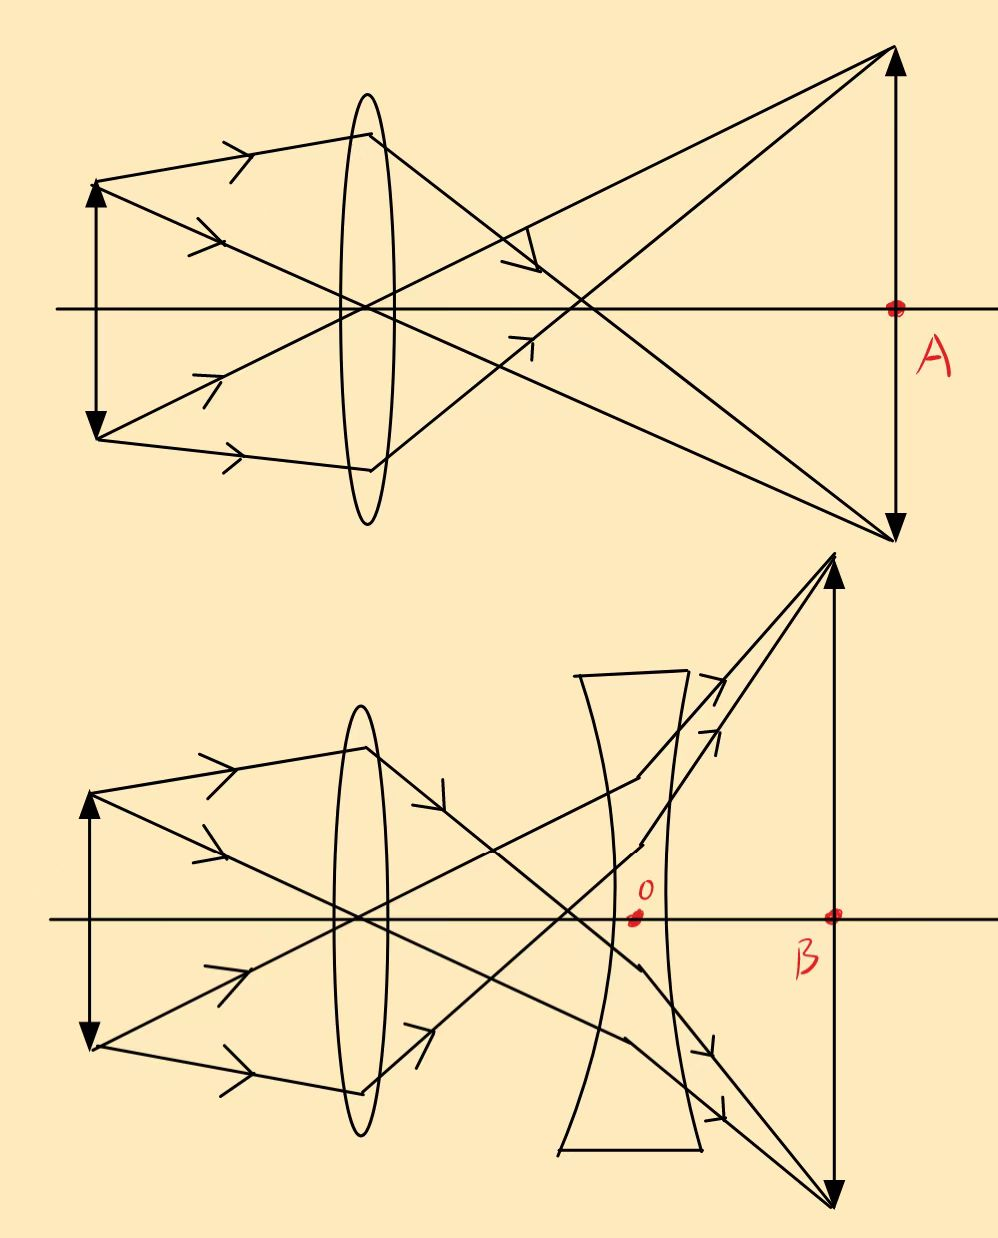
\includegraphics[width=7cm]{6.1.jpg} % 替换为你的图片路径
        \caption{测量凹透镜焦距}
    \end{figure}
\section{总结}
\hspace*{2em}在本次实验中,我们学习了测量薄透镜焦距的两种方法——自准直法和位移法,并进行了自组装显微镜、望远镜,以及估测了自组显微镜的视角放大率。在实验中,对光学系统进行共轴调节是至关重要的一步,这决定了能否看到清晰的象以及实验结果的准确性,这为日后的实验提供了宝贵的经验。

\end{document}